\documentclass[tikz]{standalone}
\usetikzlibrary{patterns, decorations.pathreplacing}

\begin{document}
    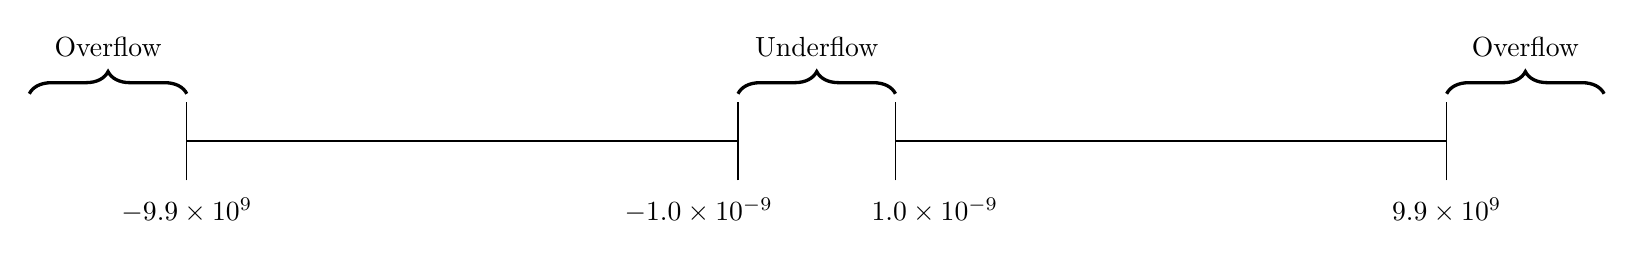
\begin{tikzpicture}
        \draw (-8,0) -- (-1,0);
        \draw (-8,-0.5) -- (-8, 0.5) node[below, yshift=-1.1cm]{$-9.9 \times 10^9$};
        \draw (-1,-0.5) -- (-1, 0.5) node[below, yshift=-1.1cm, xshift=-0.5cm]{$-1.0 \times 10^{-9}$};

        \draw (1,0) -- (8,0);
        \draw (1,-0.5) -- (1,0.5) node[below, yshift=-1.1cm, xshift=0.5cm]{$1.0 \times 10^{-9}$};
        \draw (8,-0.5) -- (8,0.5) node[below, yshift=-1.1cm]{$9.9 \times 10^9$};

        \draw[
            very thick,
            decorate,
            decoration={
                brace,
                amplitude=8pt
            }
        ] (-1,0.6) -- (1,0.6) node[midway, yshift=0.6cm]{Underflow};

        \draw[
            very thick,
            decorate,
            decoration={
                brace,
                amplitude=8pt
            }
        ] (-10,0.6) -- (-8,0.6) node[midway, yshift=0.6cm]{Overflow};

        \draw[
            very thick,
            decorate,
            decoration={
                brace,
                amplitude=8pt
            }
        ] (8,0.6) -- (10,0.6) node[midway, yshift=0.6cm]{Overflow};
    \end{tikzpicture}
\end{document}